\chapter{Graph Theory and Computational Social Science}\label{ch:GraphTheory}

Graph theory is the study of mathematical structures, called graphs, which are
used to model pairwise relations between entities. Graphs consist of a finite
set of vertices, $V$, and a set of ordered pairs of vertices, $E$, called edges.
A graph can be defined by the tuple, $G=(V,E)$. The graphs built in this project
have added constraints which are defined below:

\begin{itemize}
    \item \emph{Vertices}: Let $V_{1}=\{v_{1},v_{2},...,v_{n}\}$ be the set of
    party leaders; $V_{2}=\{v_{1},v_{2},...,v_{m}\}$ be the set of tweets by the
    party leaders described in section \ref{sec:motivation}; and let
    $V_{3}=\{v_{1},v_{2},...,v_{k}\}$ be the set of ``generic users'' who
    retweet tweets. Let the total set of vertices $V=V_{1}\cup V_{2}\cup V_{3}$.
    
    \item \emph{Edges}: Let $E$ be the set of edges. Allow the edge $(v_{1},
    v_{2})\in E$ if and only if $v_{1}\in V_{1}, v_{2}\in V_{2}$ or $v_{1}\in
    V_{3}, v_{2}\in V_{2}$. By this definition, we will only allow edges from a
    party leader vertex to a tweet vertex, or from a generic user vertex to a
    tweet vertex.
\end{itemize}

Figure \ref{fig:og_graph} shows the full graph -- with 7,978 tweets, 36,450
generic users, and 113,293 retweet edges --  built with these constraints.

\begin{singlespacing}
    \begin{figure}[H]
    \centering
    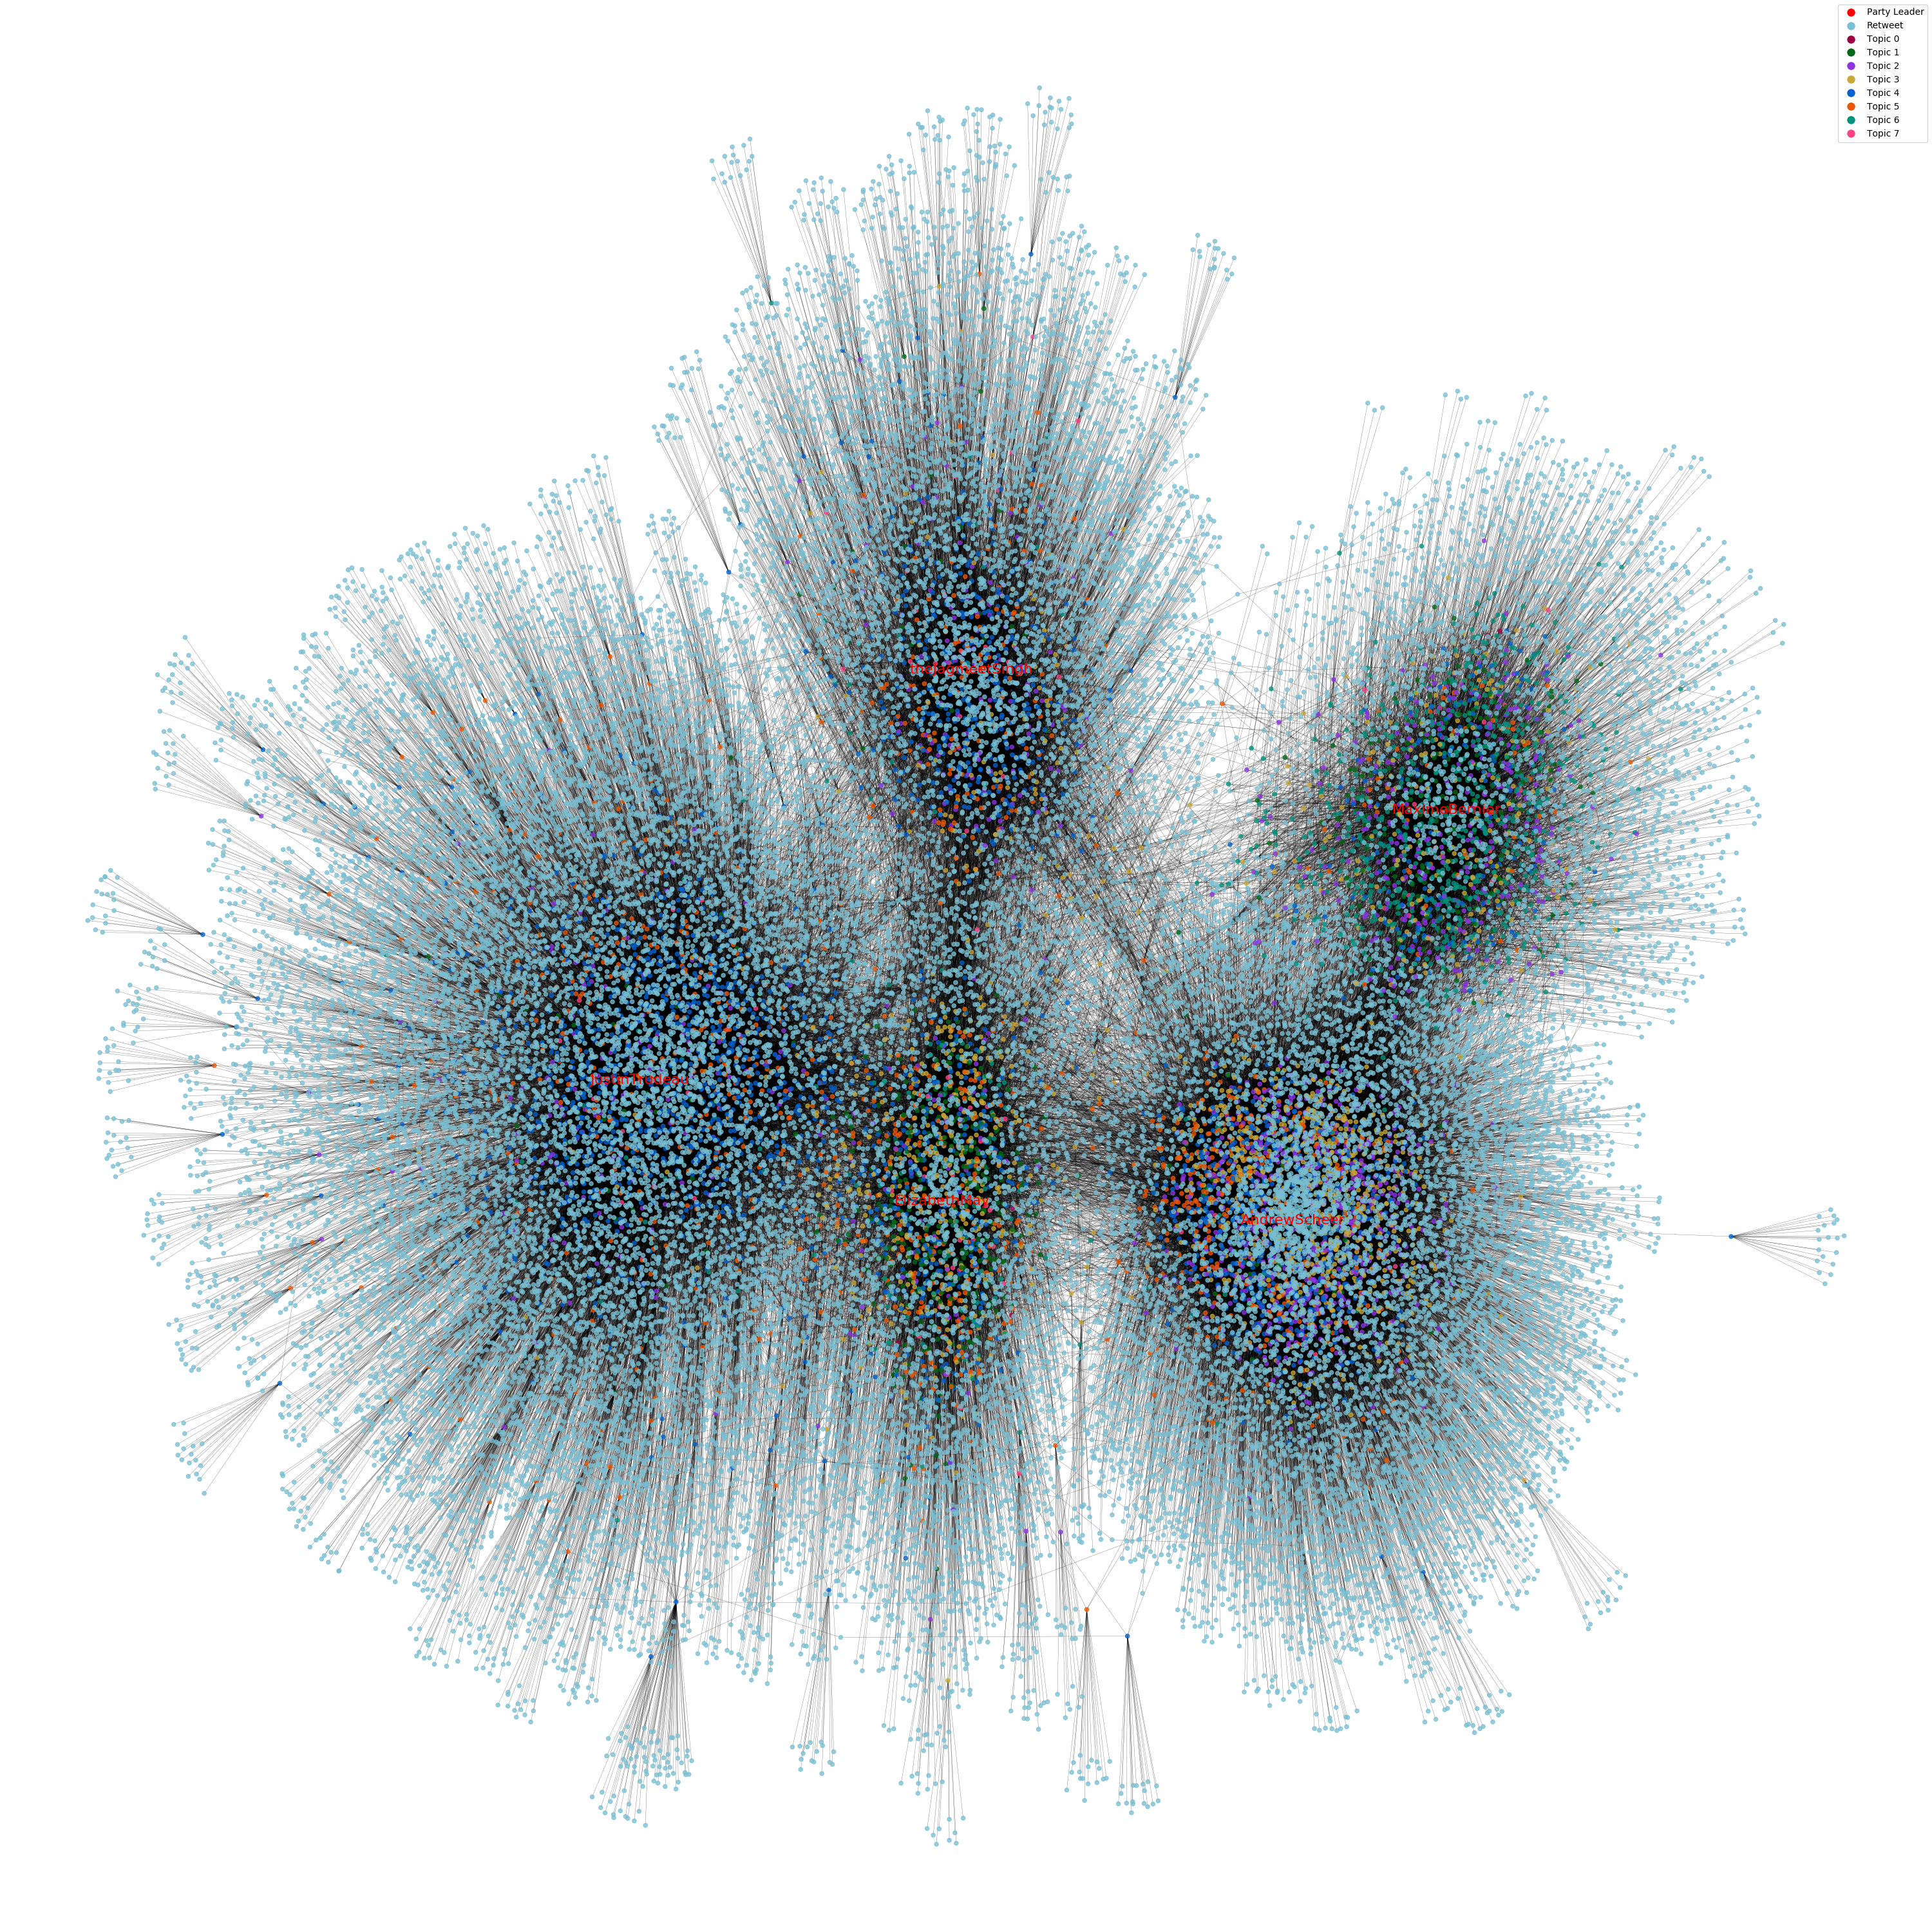
\includegraphics[scale=0.15]{Figures/og_graph}
    \caption[Complete Political Engagement Graph]{Complete Political Engagement Graph}
    \label{fig:og_graph}
    \end{figure}
\end{singlespacing}

\section{Random Graphs}\label{sec:RandomGraphs}
    
Real world interactions are not deterministic. That is -- who your friends are,
whether you contract a disease, or whether you choose to retweet a tweet are the
result of random processes, patterned by your connections with others.
Therefore, modelling how social networks form requires investigating the
underlying of the processes that generate these random ties. As Robins'
discusses in his article,\emph{ a tutorial on methods for the modeling and
analysis of social network data}, graphs where edges are generated in some
stochastic process can help illustrate how relationships drive behaviour
\cite{robins2013tutorial}.  

\subsection{Blockmodels}\label{sec:SBM}

Initially, random graph models were developed to ``model  variations in local
connectivity of each network actor, the degree of local clustering among actors,
and the general distribution of connectivity." \cite{robins2013tutorial} That
is, random graphs initially attempted to model dynamics by calculating the
probabilities of edges occurring based on where vertices were situated within
the network. However characteristics intrinsic to actors, external to their
position in a network, often pattern their relationships with others; inter vs
intra-family dynamics drive Shakespeare's play Romeo and Juliet.
\cite{doreian2005generalized}. Blockmodels were developed to take into account
the characteristics of vertices in determining edge probabilities. Blocks are
defined as all vertices with the same characteristics. The proportion of all
possibles edges within a block -- and the proportion of all possible edges that
span to all other blocks -- formulate the probabilities of forming edges in the
generative blockmodel. Figure \ref{fig:blockmodel_ex} visualizes a friendship
network with each vertex (representing a person) coloured according to their
sex, and edges between vertices denoting friendship between them.

\begin{singlespacing}
    \begin{figure}[H]
    \centering
    \includegraphics[scale=0.2]{Figures/blockmodel_ex}
    \caption[Friendship Blockmodel With Vertices Coloured by Sex]{Friendship Blockmodel With Vertices Coloured by Sex}
    \label{fig:blockmodel_ex}
    \end{figure}
\end{singlespacing}

Of all the possible edges for a network of that size, the ones observed are
overwhelmingly between members of the same sex, with fewer edges spanning that
characteristic. This is an example of an attribute, intrinsic to the actor, that
shapes behaviour which blockmodels attempt to capture. 

\subsubsection{Stochastic Blockmodels}

Stochastic blockmodelling, first proposed by Holland et al. in 1983, is a subset
of blockmodels that takes classes of vertices to be latent
\cite{holland1983stochastic}. The goal, therefore, of stochastic blockmodels are
to determine the latent classes necessary to define the blockmodel. 

For the purposes of this thesis, stochastic blockmodels will be adapted and
extended to capture how users on Twitter show preferences for party leaders
and/or policies when deciding whether to engage with tweets. The model will have
to realistically model the spectrum of users; from those who only engage with
one party leader, to those who retweet multiple party leaders, to those whose
engagement is driven by specific issues. 

\section{Spectral Graph Theory}\label{sec:spectralGraphTheory}

Spectral graph theory studies the structures of graphs via the eigenvectors of
their adjacency matrix, Laplacian matrix\footnote{The Laplacian matrix of a
graph is defined as its degree matrix minus its adjacency matrix.}, or some
other variant of the two. The set of eigenvalues for a graph of size $n$,
$\{\lambda_{1},...,\lambda_{n}\}$, is called the spectrum of a graph
\cite{netlsd}. As Hammond et al. note, graph spectra are closely related to
major graph invariants \cite{chung1997spectral}. Graph spectra have been used in
image segmentation and object recognition tasks, as well as in studying the
stability of molecules; Elghawalby and Hancock demonstrated how the euclidian
distance between graphs' spectra track the edit distances between graphs
\cite{elghawalby2008measuring,chung1997spectral}. As such, spectral graph theory
is useful in comparing the underlying structure of two graphs -- allowing for
nuanced distance and similarity metrics.   

\subsection{Network Laplacian Spectral Descriptor}\label{sec:NetLSD}

While various distance metrics are tracked by graph spectra, most are not size
invariant or scale adaptive. Size invariant similarity metrics capture two
structurally similar graphs as close together, regardless of magnitude; for
example, social networks like Facebook and Google Hangout likely have similar
structural patterns despite the former being much larger. Scale adaptive
similarity metrics would be able to capture both local and global features of a
graph. To solve this, Tsitsulin et al. developed the Network Laplacian Spectral
Descriptor (NetLSD), which extracts a compact heat trace signature from a
graph's normalized Laplacian spectrum using the heat kernel \cite{netlsd}. This,
in effect, models how heat diffuses throughout a network over time; with local
features being captured in the immediate time-steps after the vertices are
``heated'' (and only affecting adjacent vertices) and global features being
captured as heat becomes further diffuse. Figure~\ref{fig:heat_trace_ex} shows
how the two graphs can be similar at a global level and local level, but differ
at an intermediate scale \cite{netlsd}.

\begin{singlespacing}
    \begin{figure}[H]
    \centering
    \includegraphics[scale=0.25]{Figures/heat_trace_ex}
    \caption[NetLSD Heat Trace Signatures for two Similar Graphs \cite{netlsd}]{NetLSD Heat Trace Signatures for two Similar Graphs \cite{netlsd}}
    \label{fig:heat_trace_ex}
    \end{figure}
\end{singlespacing}

The heat trace ($h_{t}$) for a graph at time $t$ is calculated by taking the
eigenvalues of the graph's normalized Laplacian matrix, and summating their
exponentiation multiplied by $-t$. 

\begin{equation}\label{equation:heat_trace}
    h_{t}=\sum_{j}^{n}e^{-t\lambda_{j}}
\end{equation}
 
Given that a graph with $n$ vertices will have $n$ eigenvalues and thus larger
graphs may tend to have higher heat trace values at any given time -- the heat
trace can be normalized against an empty graph of size $n$, which has all zero
eigenvalues \cite{netlsd}. The \emph{heat trace signature} then is a vector of
different heat traces at different times denoted by $h(G)$:

\begin{equation}\label{equation:heat_trace_sig}
    h(G) = \{h_{t}\}_{t\geq0}
\end{equation}

Since the heat trace signatures of two graphs lie in the same dimensional vector
space, taking the $L_{2}$ distance of the difference between the signatures
provides a suitable distance metric.
	
\section{Measures of Centrality}

Centrality is a measure of prominence for vertices within a graph. For the
purpose of this thesis, it will be used to measure the relative importance of
different topics tweeted about in the lead up to Canada's 2019 federal election.

\subsection{Background}\label{sec:CentralityBackground}

There are various different ways of measuring vertex centrality that have
successfully been applied to problems in marketing, economics and epidemiology;
Stephenson and Zelen explored the utility of centrality measures in studying the
social dynamics of Gelada baboons. \cite{stephenson1989rethinking}. Common
centrality measures include measures of degree and betweenness. This thesis will
focus on the notion that central vertices are close to other central vertices,
which is one of the founding intuitions behind Google’s “page-rank” algorithm
and eigenvector centrality. 

\subsection{Eigenvector Centrality}\label{sec:EigCentrality}

As Newman lays out in his 2016, Mathematics of Networks: ``the eigenvector
centrality [...] accords each vertex a centrality that depends both on the
number and the quality of its connections: having a large number of connections
still counts for something, but a vertex with a smaller number of high-quality
contacts may outrank one with a larger number of mediocre contacts.''
\cite{newman2008mathematics}

The eigencentrality of vertex $x$ is defined as $C_{E}(x)$, where $C_{E}(x)$ is
proportional to the average eigenvector centrality of $x$'s neighbours,
multiplied by some constant $\lambda$:
\begin{equation}
    C_{E}(x)=\frac{1}{\lambda}\sum_{j=1}^{n}A_{xj}C_{E}(x)
\end{equation}
By defining the vector of centralities as $C_E(X) = (C_E(x_1),C_E(x_2),...)$
this equation can be rewritten as $\lambda C_E(X) = \lambda A$, and it is
evident that $C_E(X)$ is an eigenvector of the adjacency matrix with eigenvalue
$\lambda$ \cite{newman2008mathematics}. By Perron-Frobenius theorem, picking the
largest eigenvalue of $A$ will result in all elements of $C_E(X)$ being
non-negative \cite{newman2008mathematics}.